\chapter{Docker}

Docker soll es Entwicklern vereinfachen, Container für Applikationen zu erstellen, zu verteilen und sie auf verschiedensten Systemen auszuführen. Es hilft dabei Applikations-Container zu erstellen \cite{docker}, die später in einem einzelnen Prozess auf verschiedenen Systemen ausgeführt werden können. Die erste Version wurde im März 2013 von dotCloud veröffentlicht (jetzt Docker, Inc.) \cite{docker:rel}.
Docker basierte bis zu Version 0.9 \cite{docker:cl} auf dem Container-Standard LXC und erweiterte diese vor allem durch eine einfachere Handhabung. So können Images durch einfache Konfigurationsdateien definiert werden und über die Docker API erstellt und verwaltet werden. Beim Starten eines Containers können diese mit anderen verbunden werden, um so die Kommunikation der eigentlich voneinander isolierten Container zu vereinfachen und über andere Tools können ganze Cluster von Docker-Containern verwaltet werden.

\paragraph{}
Über eine Docker-Registry ist es möglich Container Images zu versionieren und zu teilen. Die Docker-Registry kann wie Git für Container gesehen werden.  Bei dem Bau neuer Container Images kann man so immer wieder auf sogenannte Base-Images zurückgreifen, die man in einer Docker-Registry findet und auf denen man seine eigenen Images aufbauen kann.

\paragraph{}
LXC ist dabei nur ein Tool um Container zu erstellen und zu starten und Docker vereinfacht die Verwaltung dieser Container. Mit “libcontainer” implementierte Docker Inc. eine eigenen Container-Standard, um die starken Abhängigkeiten von LXC aufzulösen. Daraus ging die “Open Container Initiative”, die OCI (https://www.opencontainers.org/) und “runC” (http://runc.io/) hervor. Die OCI ist ein Zusammenschluss mehrerer großer Firmen, angeführt von Docker, mit dem Ziel, einen einheitlichen offenen Container Standard zu definieren. Anhand dieser Spezifikation können Container dann auf verschiedenen Systemen implementiert werden und von Systemen wie Docker einheitlich verwaltet werden. runC ist dabei die Implementation der Spezifikationen der OCI und ersetzt LXC.

% ------------
% -- Engine --
% ------------

\section{Docker Engine}

Die Docker Engine ist eine Client-Server Anwendung, die auf dem Host-System installiert wird und besteht aus drei Hauptbestandteilen:\\

\begin{itemize}
  \item dem Docker Daemon (der Server), der für das Erstellen und Ausführen der Container zuständig ist
  \item der Docker Remote Api für die Kommunikation zwischen Client und Docker Daemon
  \item der CLI (Command Line Interface)
\end{itemize}

\begin{figure}[!ht]
  \centering
  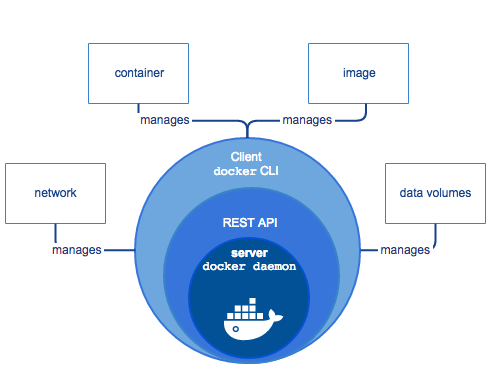
\includegraphics[width=0.5\textwidth]{images/8-docker-engine.png}
  \caption{Die drei Hauptbestandteile der Docker-Engine \cite{docker:ud}}
\end{figure}

Die Client-Server Architektur ermöglicht es einerseits Client und Daemon auf verschiedenen Hosts laufen zu lassen und so auch Container auf anderen Servern zu verwalten, andererseits kann der Daemon durch die API über einen beliebigen Client gesteuert werden. Das können andere Sprachen wie beispielsweise Python sein, für die eine vollständige Docker-Api-Implementation vorliegt oder auch grafische Benutzeroberflächen.

% --------------------------
% -- Images and Container --
% --------------------------

\section{Images und Container}

Ein Docker Container wird auf Basis eines Docker Images gebaut. Jedes Docker Image besteht aus mehreren Layern, einem Base Image und welchen, die das Image jeweils um Funktionen erweitern, die für das Ausführen einer Applikation wichtig sind. Die Layer liegen dabei in jeweils eigenen Verzeichnissen und werden über ein “unified view” zu einem einzelnen Image zusammengefasst. Ein “unified view” kann als virtuelles Verzeichnis gesehen werden, in dem die einzelnen Layer so übereinandergelegt werden, dass die verschiedenen Layer von oben als einzelnes Image gelesen werden können. Existiert in einem Layer die gleiche Datei wie in dem Base Image mit einer anderen Konfiguration, so verdeckt diese die Datei aus dem Base Image.\\

\begin{figure}[!ht]
  \centering
  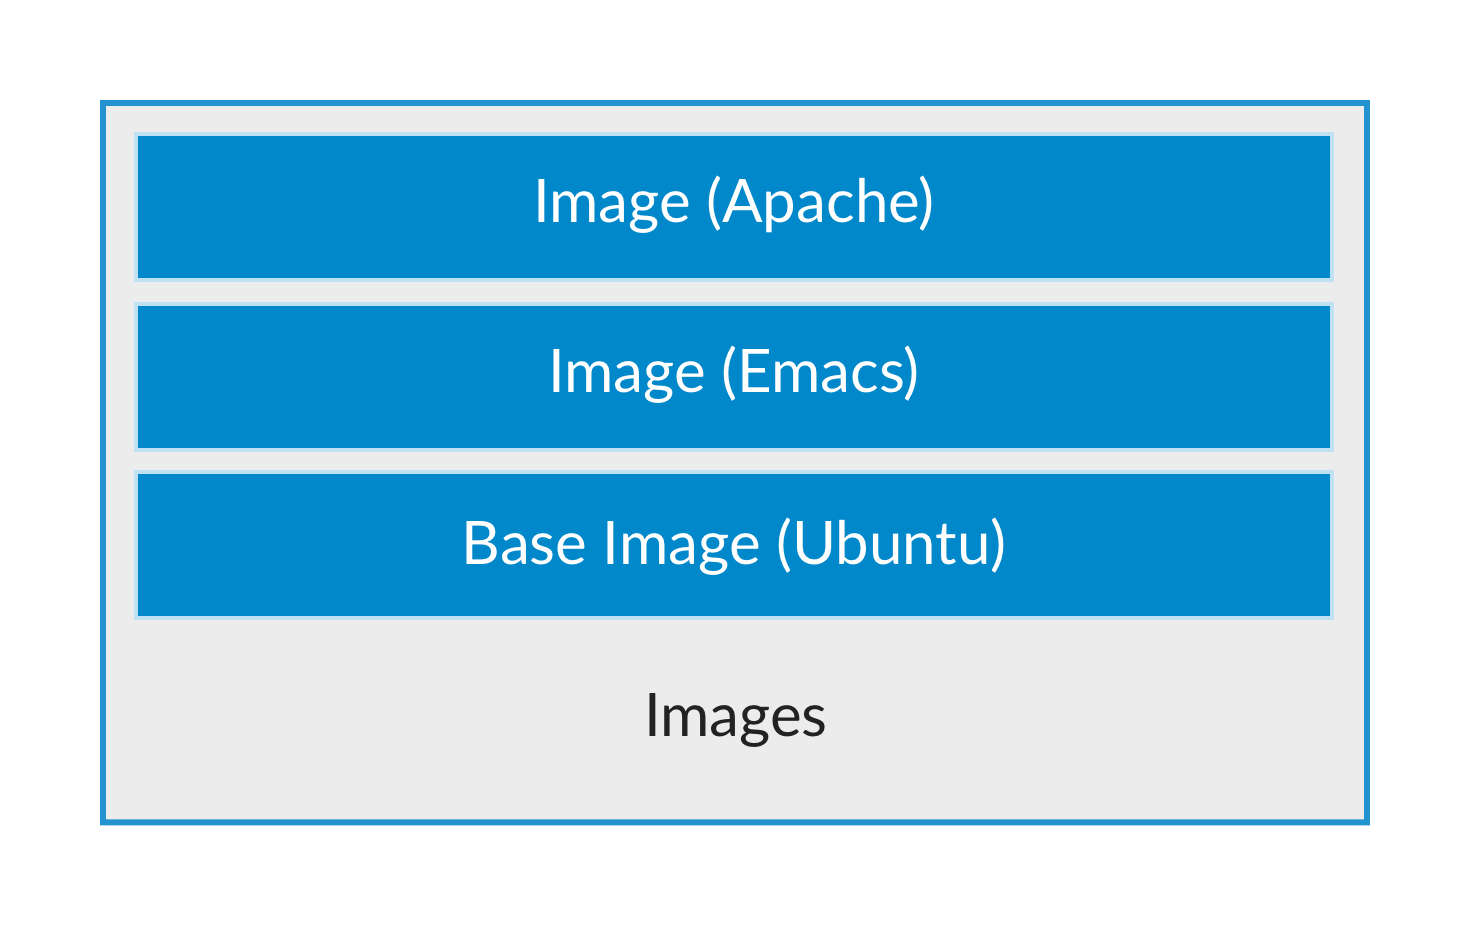
\includegraphics[width=0.6\textwidth]{images/9-docker-image.png}
  \caption{Ein Image bestehend aus mehreren übereinandergestapelten Layern \cite{7158965}}
\end{figure}

Die einzelnen Layer in einem Image sind nur lesbar, können also nicht mehr verändert werden. So können die Layer von beliebig vielen Images verwendet werden. Jeder Layer hat einen eindeutigen Hash und kann gezielt von verschiedenen Images verwendet werden und es kann sichergestellt werden, dass der Layer immer genau gleich ist. Das bedeutet, dass der Layer nur ein einziges Mal im Dateisystem gespeichert werden muss. Über die “unified view” werden die Layer anschließend in den Images verwendet. So können die Layer von beliebig vielen Images verwendet werden bei konstantem Platzverbrauch. Jede Änderung an einem Image fügt dem Image einen Layer hinzu. Jeder Layer steht dabei für Unterschiede im Dateisystem im Bezug auf die übrigen Layer. Das können nur einzelne Konfigurationsdateien sein, sodass die Größe des Layers nur wenige Bytes beträgt, aber auch ganze Programmpakete, die deutlich mehr Platz benötigen.\\

\begin{figure}[!ht]
  \centering
  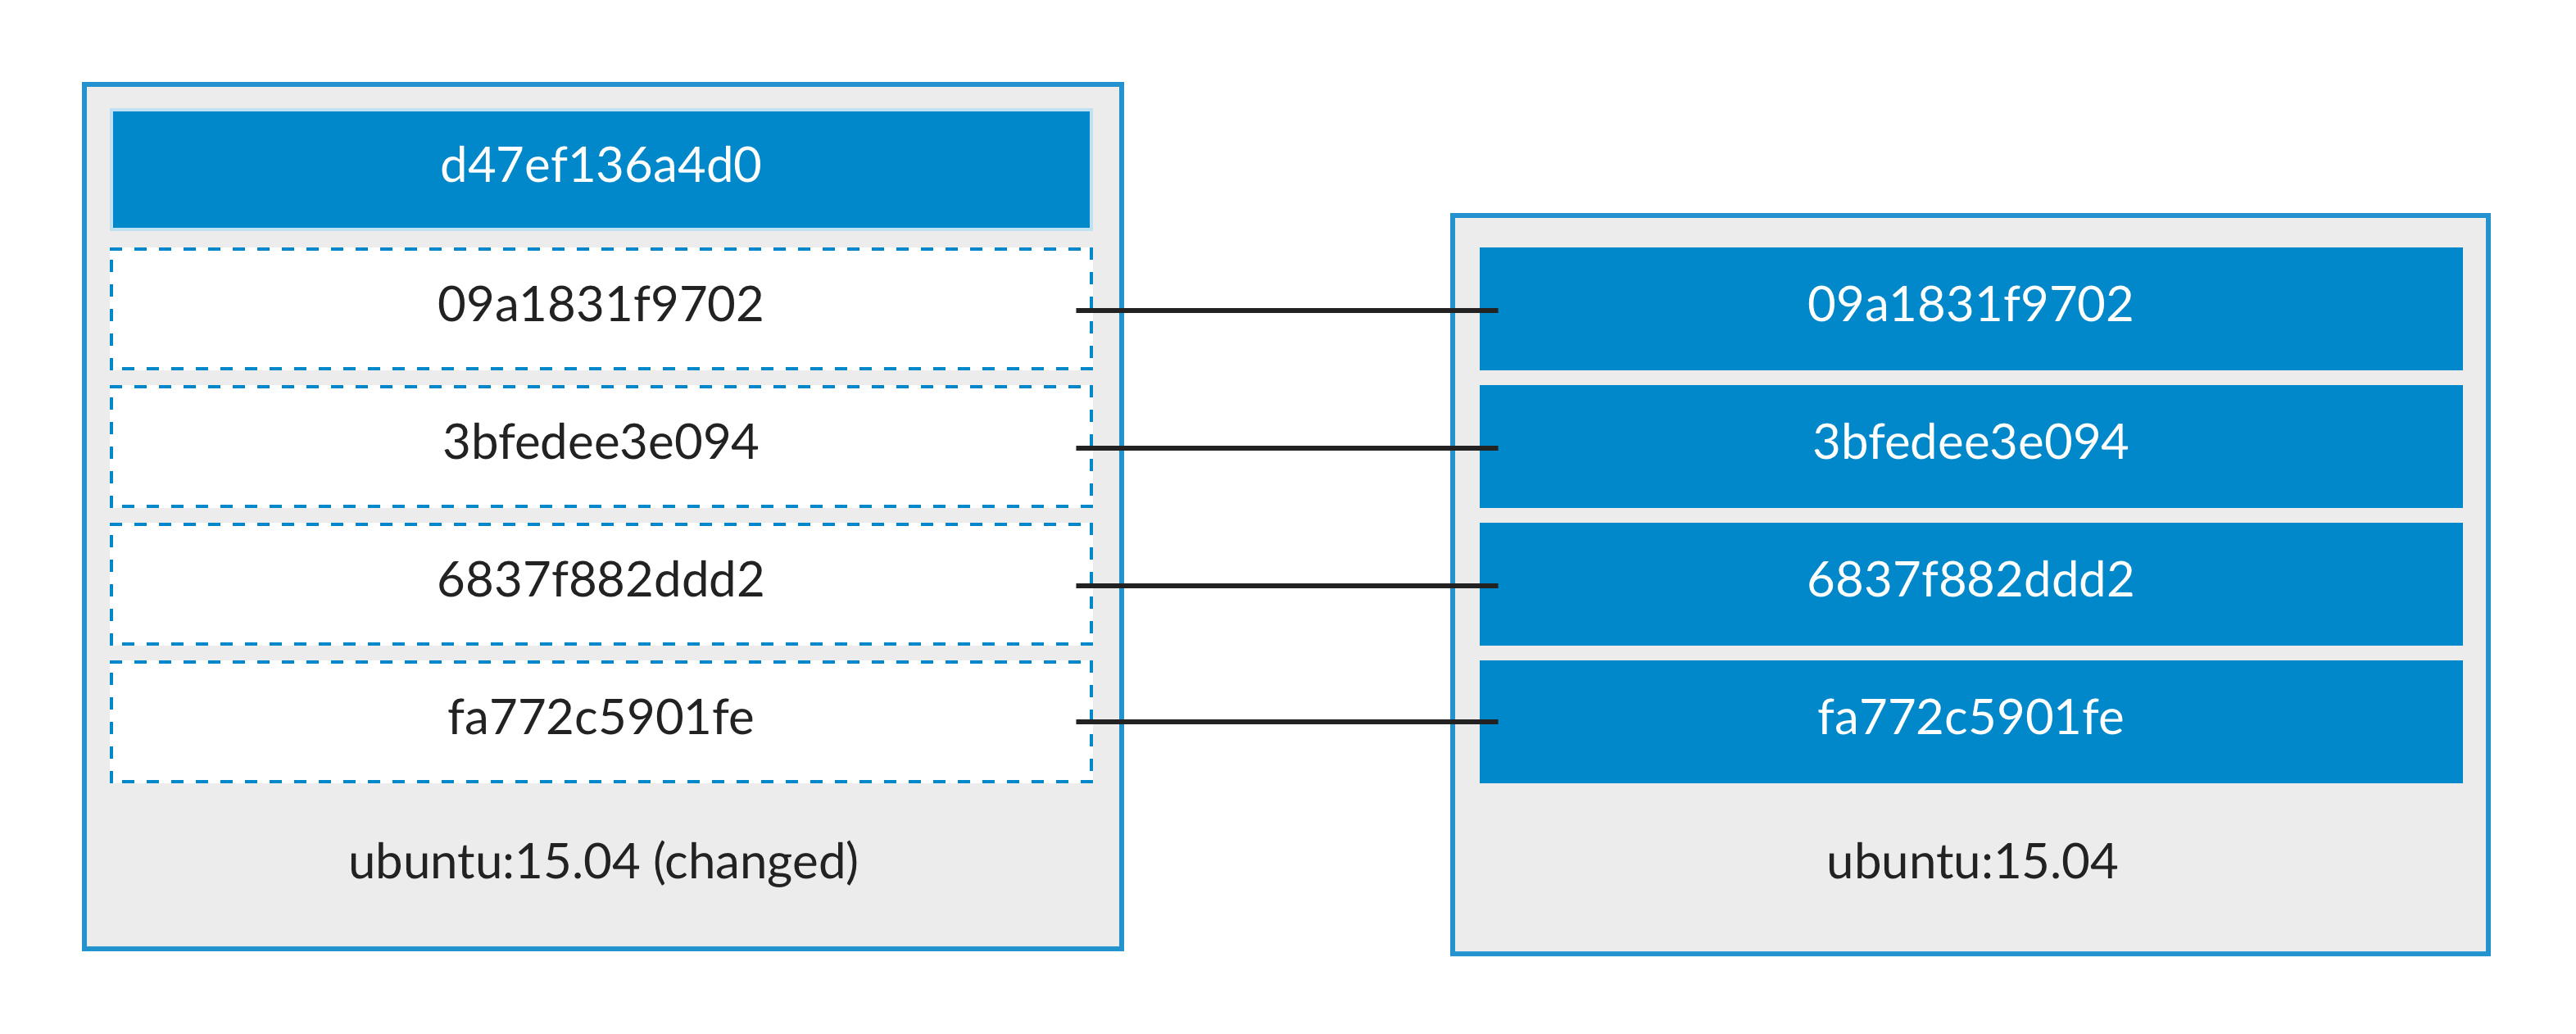
\includegraphics[width=1\textwidth]{images/10-docker-image-layer-sharing.png}
  \caption{Ein Image mit neuem Layer, dass die ursprünglichen Layer mit verwendet \cite{docker:images}}
\end{figure}

Bei der Erstellung eines Containers aus einem Image wird nach dem gleichen Prinzip dem ursprünglichen Image nun ein “Container-Layer” hinzugefügt, der im Gegensatz zu den übrigen beschreibbar ist. Ist der Container gestartet, werden alle Dateiänderungen in den diesen Layer geschrieben. Dafür ist neben dem “Unified View” ist noch ein weiteres Verfahren, das “copy-on-write” Verfahren wichtig. Während die Container laufen, arbeiten beliebig viele Container mit den gleichen Original-Dateien aus dem jeweiligen Layern. Da diese nur gelesen werden können, können diese entsprechend nicht von den jeweiligen Containern modifiziert werden. Deshalb werden diese Dateien, sobald sie verändert werden sollen aus dem jeweiligen Read-Only Layer in den Container-Layer kopiert, wo sie entsprechend bearbeitet werden können.
Der Container, der die Datei bearbeitet hat arbeitet danach mit seiner Kopie im Container-Layer, während die übrigen Container weiter mit dem Original arbeiten. Dadurch können beliebig viele Container platzsparend zur gleichen Zeit laufen \cite{docker:images}.\\

\begin{figure}[!ht]
  \centering
  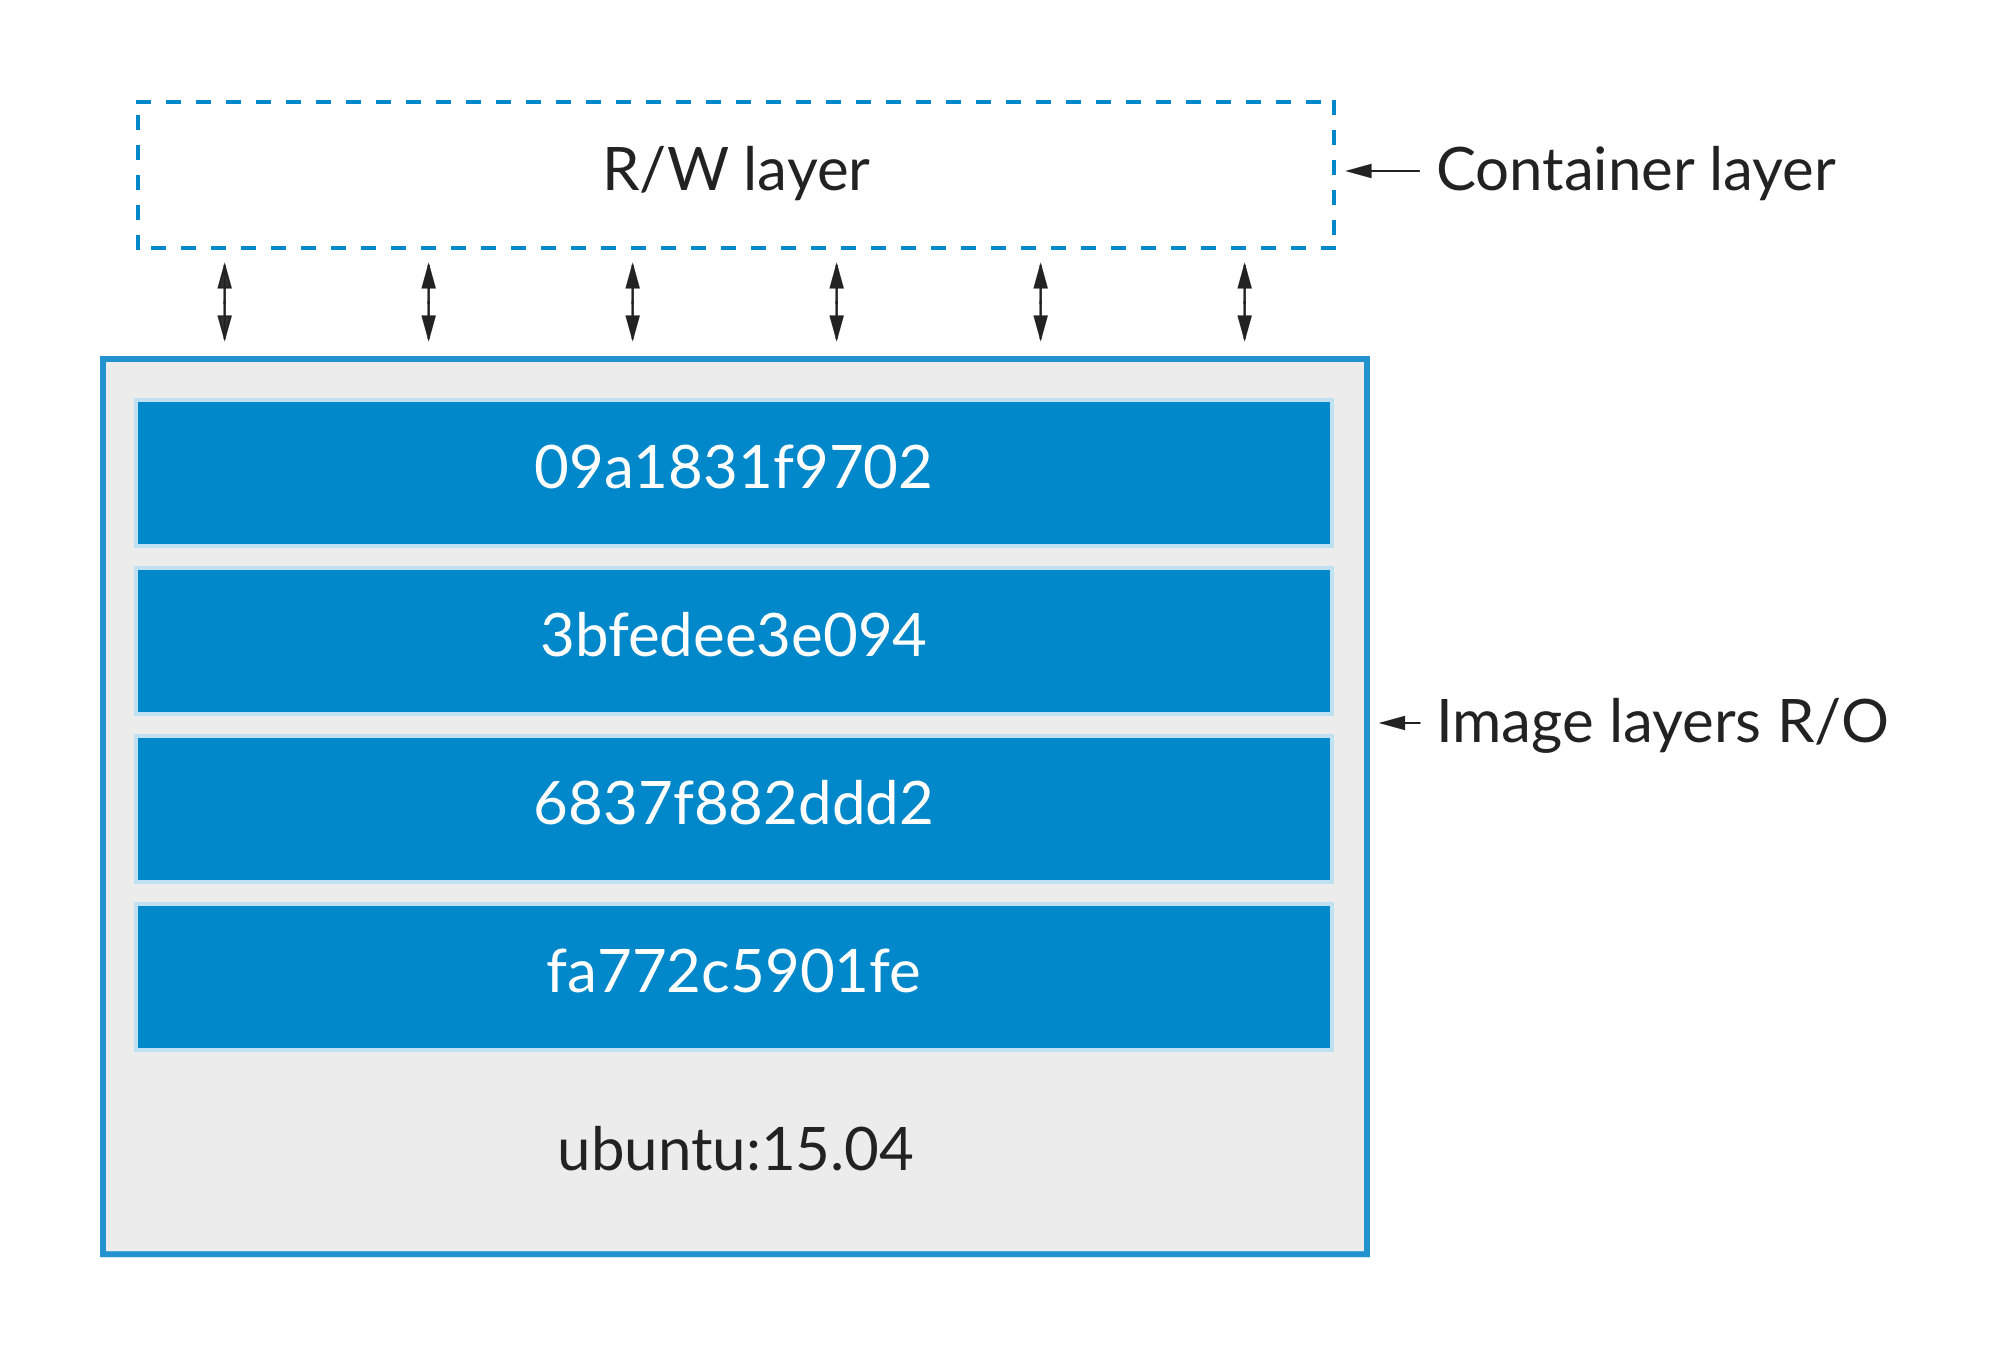
\includegraphics[width=0.8\textwidth]{images/11-docker-container.png}
  \caption{Ein Container, bestehend aus R/O Image Layern und R/W Container Layer \cite{docker:images}}
\end{figure}

Gesteuert werden sowohl der “Unified View” als auch “Copy-on-Write” von verschiedenen “Storage-Drivern”, die zwar unterschiedlich implementiert sind, aber auf dem gleichen Prinzip beruhen. Bei der Konfiguration von Docker, kann man zwischen verschieden Implementierungen wählen. Die bekanntesten sind wohl “auFS” und “overlayFS”.

\paragraph{}
Beim Löschen  eines Containers werden auch alle Dateien, die beim Ausführen der Applikation erstellt wurden, gelöscht. Für das Persistieren von Daten gibt es die Möglichkeit, die Container mit sogenannten Data-Volumes zu verbinden.

\paragraph{}
Definiert werden die Images über Dockerfiles. Vereinfacht fügt jeder Befehl in der Datei dem Image ein neuen Layer hinzu. Über "docker build" wird das Image entsprechend des Dockerfiles gebaut. Jedes Image kann auf bereits vorhandenen Images aufbauen. Images können in einer Docker-Registry gespeichert werden und werden bei Bedarf bei der Erstellung des Images heruntergeladen. Dabei werden bereits vorhandene Layer im Dateisystem nicht erneut heruntergeladen. Das Beispiel baut ein Image basierend auf Ubuntu, das beim Starten des Containers “Hello world” ausgibt und in eine Datei schreibt.\\

\begin{figure}[!ht]
  \centering
  \sourcecode{src/Dockerfile1}
  \caption{Ein Dockerfile}\label{figure:Dockerfile}
\end{figure}

% --------------------------
% ----- Docker Daemon ------
% --------------------------

\section{Docker Daemon}

Der Docker Daemon (dockerd\footnote{https://docs.docker.com/engine/reference/commandline/dockerd/}) ist der zentrale Bestandteil von Docker. Er ist die Schnittstelle zwischen der einfachen Handhabung von Docker und den Vorteilen Applikations-Container gegenüber normalen VMs bieten. Er setzt auf containerd\footnote{https://containerd.io/} auf, einer Ausführungsumgebung(runtime) für Container, um runC Container nach dem OCI-Standard auszuführen und zu verwalten. containerd basiert auf Dockers altem Daemon. Er setzt auf einem niedrigeren Level an und wird von dem Docker Daemon erweitert. Wird der Docker Daemon über seine API angesprochen gibt dieser die vereinfachten Befehle übersetzt an containerd weiter \cite{docker:daemon}.\\

% https://blog.docker.com/2016/04/docker-engine-1-11-runc/, https://docs.docker.com/engine/understanding-docker/
\begin{figure}[!ht]
  \centering
  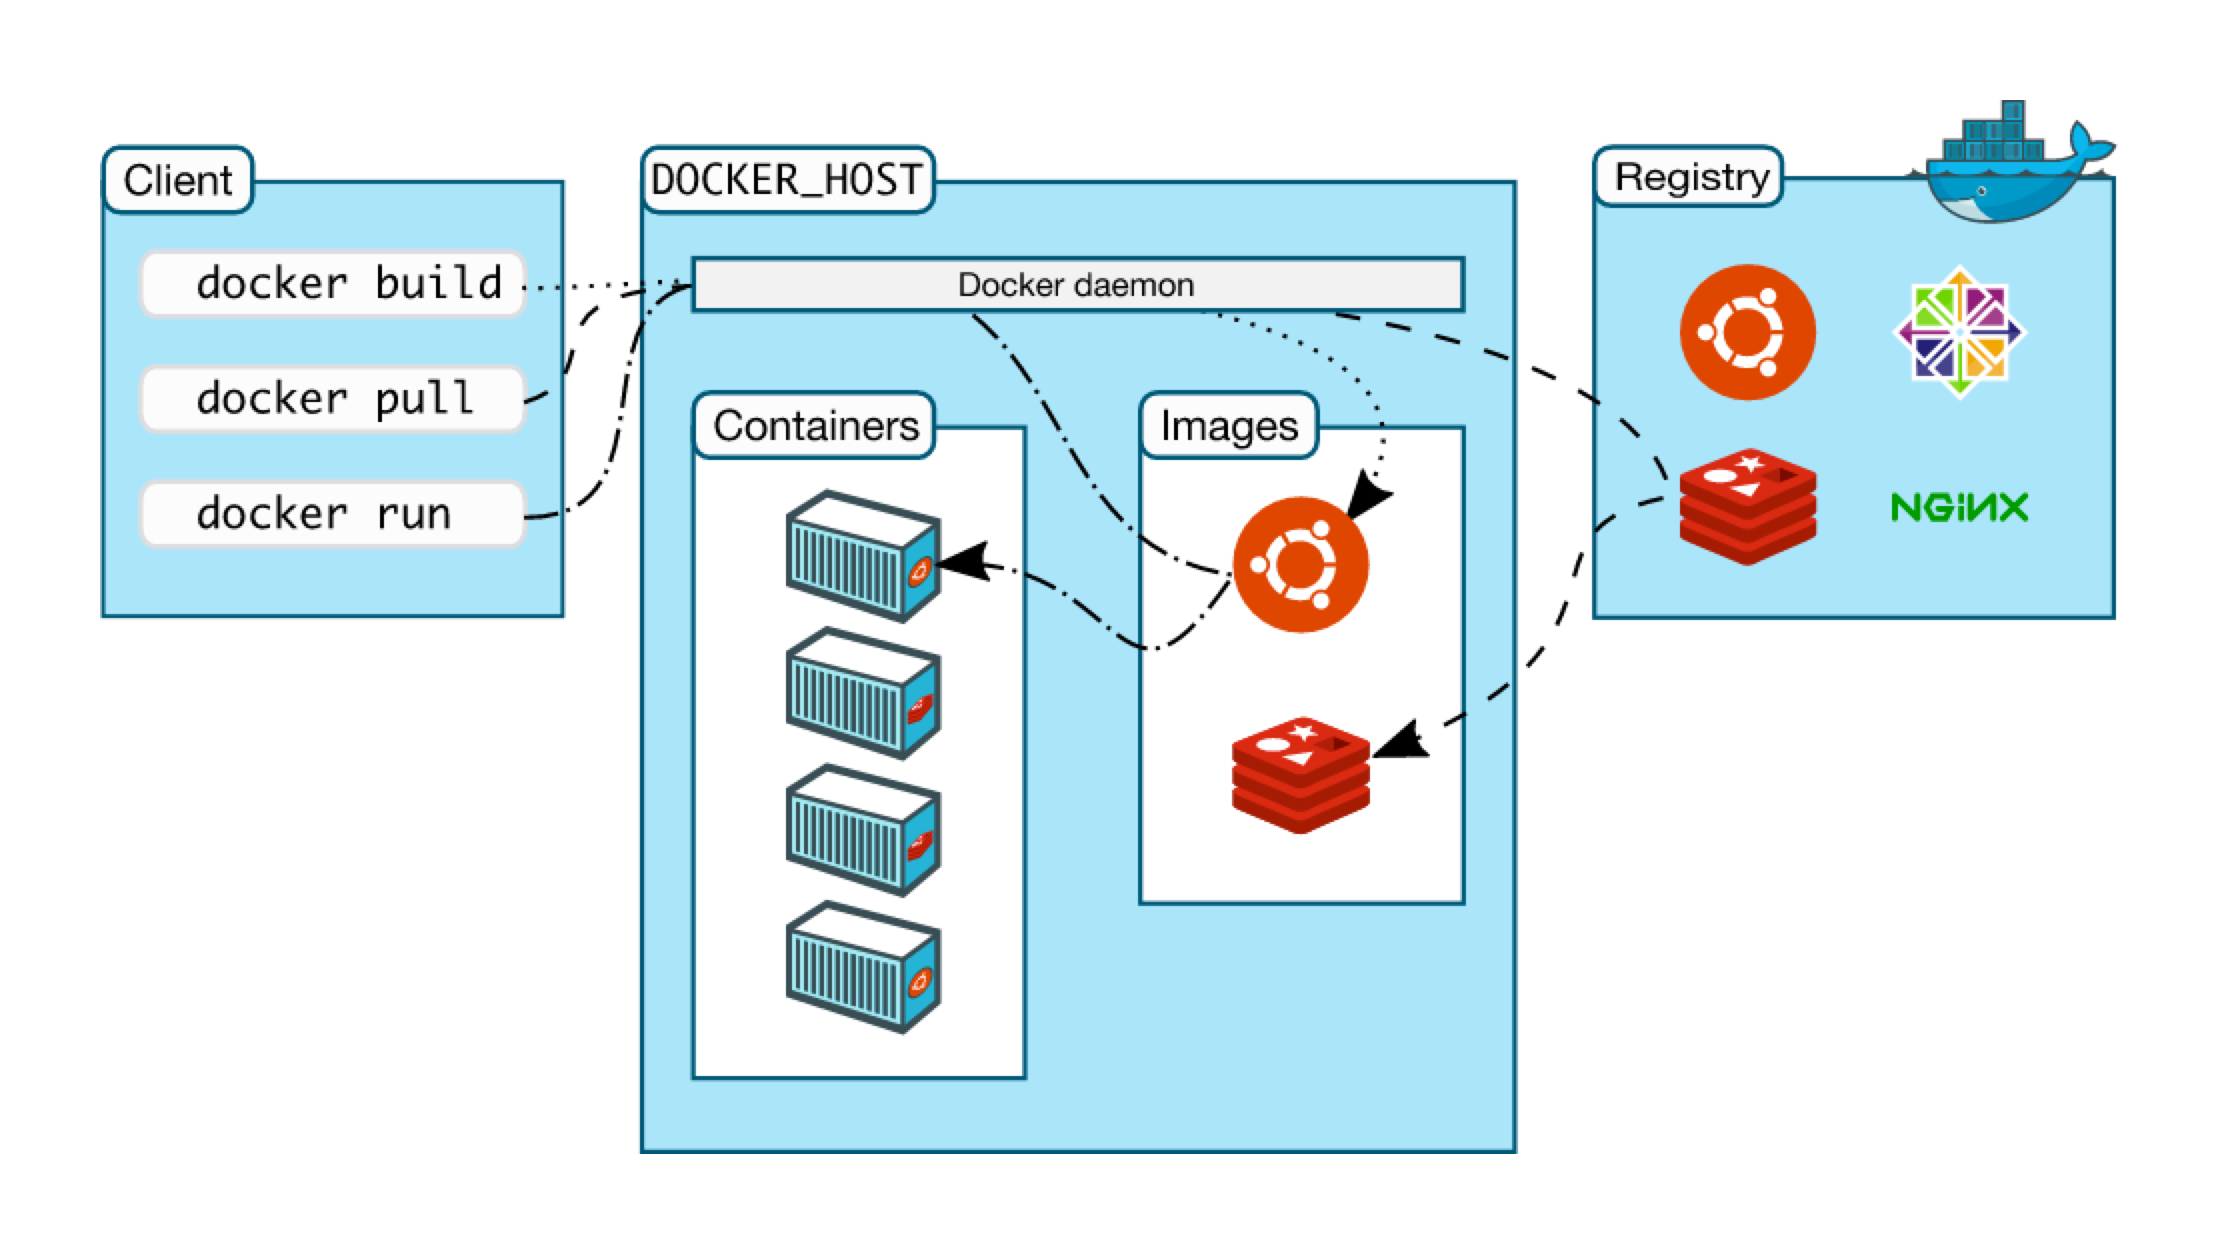
\includegraphics[width=0.8\textwidth]{images/12-docker-daemon.png}
  \caption{Docker Daemon\cite{docker:ud}}
\end{figure}

\noindent Wird zum Beispiel das Kommando \code{docker run -i -t ubuntu} ausgeführt, checkt die Docker Engine, ob das Ubuntu Image sich bereits auf dem System befindet. Ist das nicht der Fall wird das Image aus der Docker Registry gepullt und auf die Festplatte geladen. Daraus wird der Container erstellt, indem dem Image ein R/W Layer hinzugefügt wird. Danach wird das Netzwerk entsprechend konfiguriert, damit der Docker Container mit dem Host-System kommunizieren kann und dem Container wird eine IP-Adresse zugewiesen, über die der Container erreichbar ist. Zum Schluss werden die definierten Kommandos aus dem Dockerfile ausgeführt und man kann (durch das \code{-i} Flag) über das Terminal mit dem Container interagieren.

% -------------------------
% ------ Docker API -------
% -------------------------

\section{Docker API}
Über die Docker Remote API kann ein Client mit dem Docker Daemon ansprechen. Client und Daemon können sowohl auf dem gleichen Host als auch über verschiedene Hosts über die Http-Schnittstelle miteinander kommunizieren. Der Client muss dabei kein Benutzer sein, sondern können zum Beispiel Überwachungsprogramme sein. Unter anderem bietet die Docker API zum Beispiel einen Event-Stream, bei dem sich diese Programme registrieren und dementsprechend auf Zustandsänderungen reagieren können. Fällt zum Beispiel ein Container aus, können so automatisch neue Container erstellt und ausgeführt werden \cite{docker:api}.\\

\begin{figure}[!ht]
  \centering
  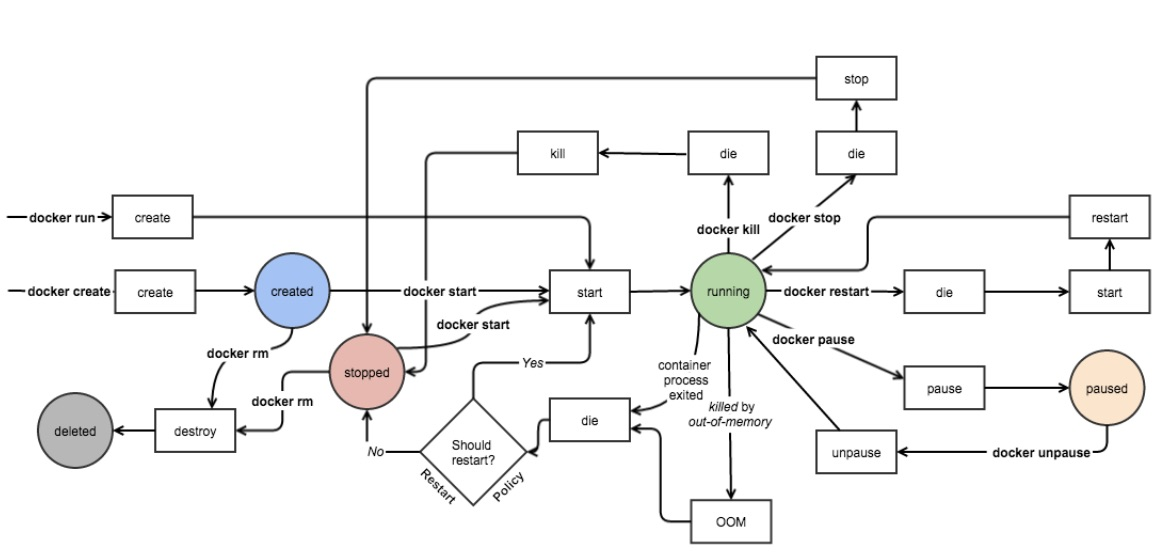
\includegraphics[width=0.8\textwidth]{images/13-docker-api.jpg}
  \caption{Die Zustände die ein Docker-Container besitzen kann und die dafür verantwortlichen Events \cite{docker:api}}
\end{figure}

% -------------------------
% ------ Docker CLI -------
% -------------------------

% \section{Docker CLI}
%
% Über die Docker CLI kann man den Docker Daemon über die Docker Remote API ansprechen. Hier einige wichtige Befehle:\\
%
% \begin{itemize}
%   \item \code{docker build}
%   \item docker run
%   \item docker build
%   \item docker start
%   \item docker push
%   % \item docker rm CONTAINER_ID
%   % \item docker rmi IMAGE_ID
%   % \item docker images
%   \item docker ps -a
%   \item ...
% \end{itemize}
